\nonstopmode
\documentclass{llncs}
\usepackage{graphicx}
\usepackage{verbatim}
\usepackage{amssymb}
\newcommand{\Butterfly}{\mbox{\large $\rhd\!\!\!\lhd$}}
\newcommand{\sync}[1]{\raisebox{-1.0ex}{$\;\stackrel{\Butterfly}{\scriptscriptstyle #1}\,$}}
\title{Bio-PEPA Model Report}
\author{Bio-PEPA Workbench}
\institute{\today}
\begin{document}
\maketitle
\section{Bio-PEPA model}
\input{example_classes_biopepa}
\begin{figure}[htbp]
\begin{center}
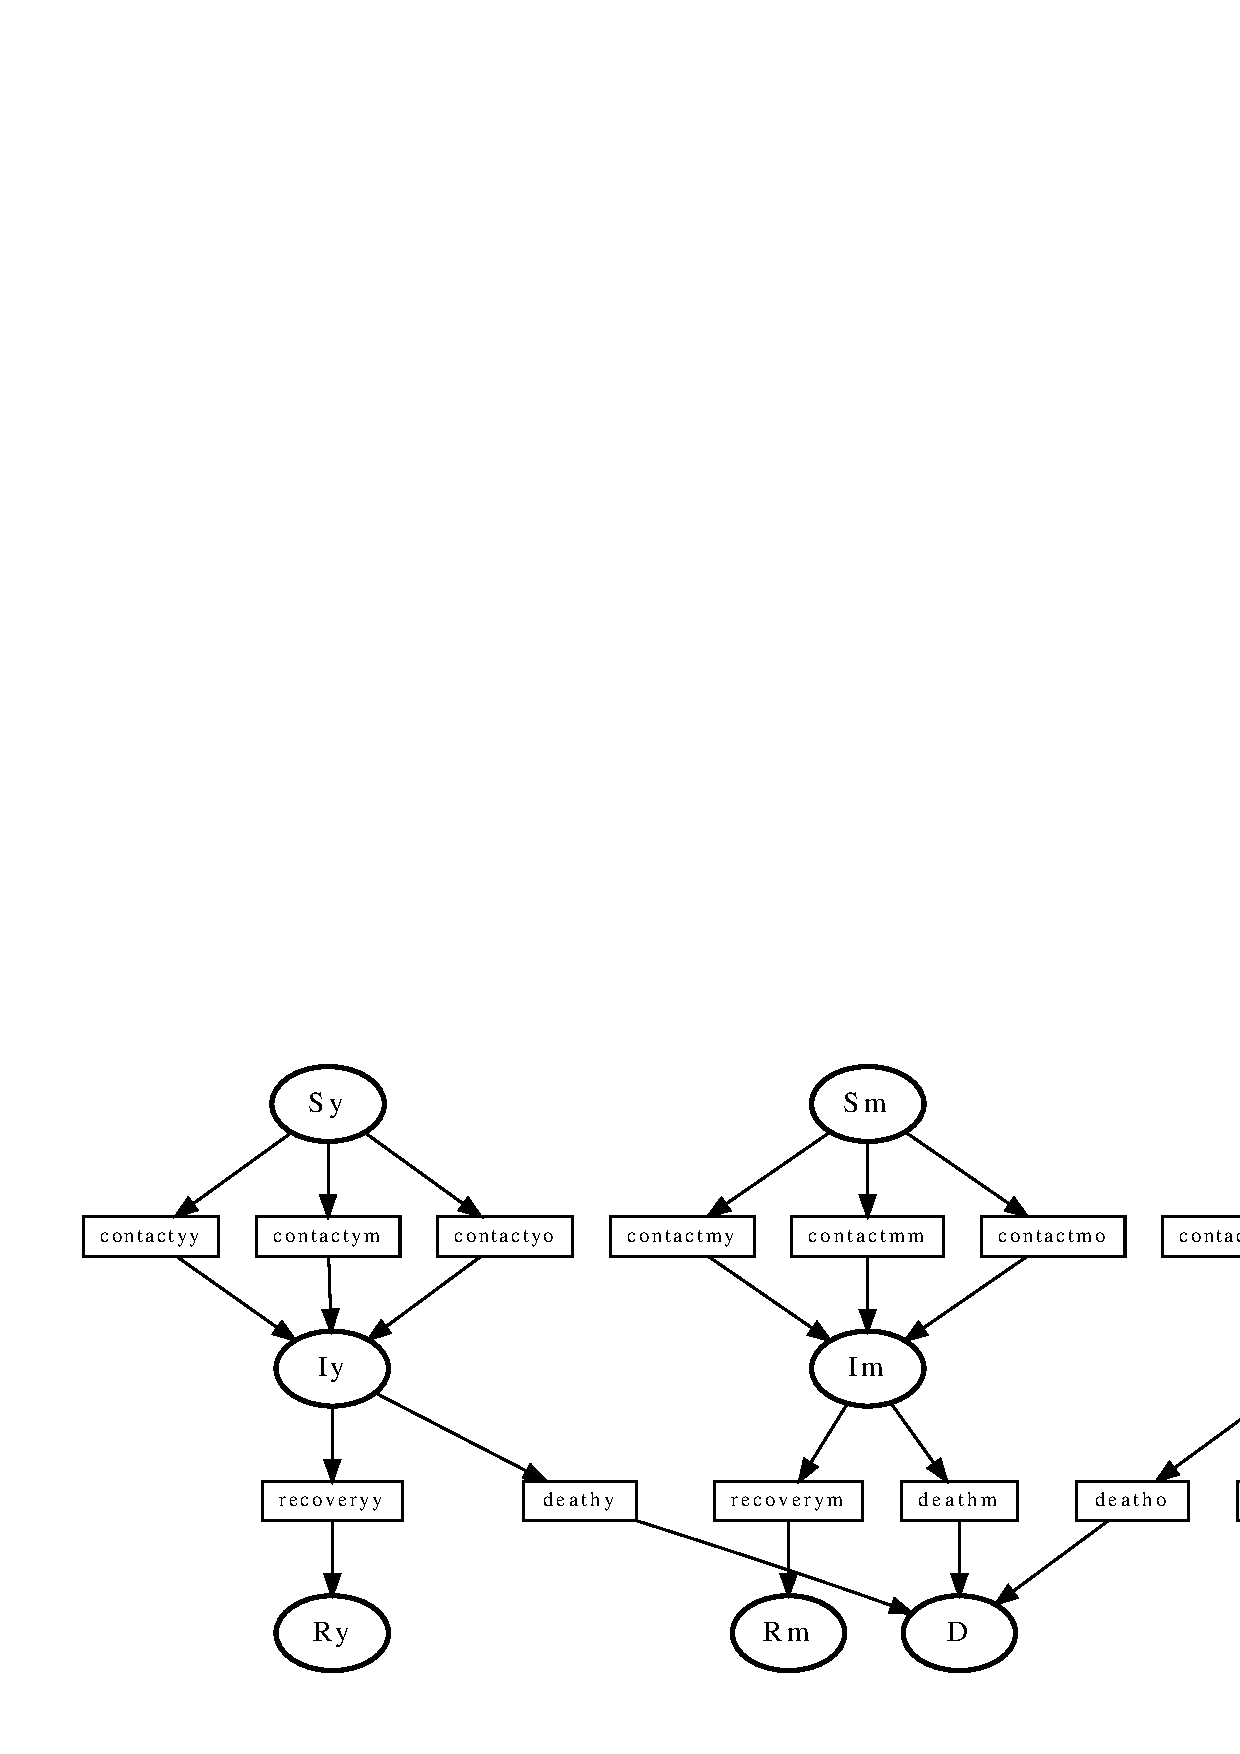
\includegraphics[width=0.6\textwidth]{dot/example_classes.pdf}
\caption{Reaction network}
\end{center}
\end{figure}
\newpage
\section{Graphs from Bio-PEPA model}
\includegraphics[scale=0.5]{png/example_classes001_dizzy_results_0}
\hfill
\includegraphics[scale=0.5]{png/example_classes001_dizzy_results_1}
\appendix
\newpage
\section{Bio-PEPA input file}
\verbatiminput{example_classes.biopepa}
\newpage
\section{Dizzy equivalent input file}
\verbatiminput{dizzy/example_classes001.dizzy}
\newpage
\section{PRISM equivalent input file}
\verbatiminput{prism/example_classes001.sm}
\end{document}
